	\pagestyle{euclidprob}
    \begin{figure}[h]
        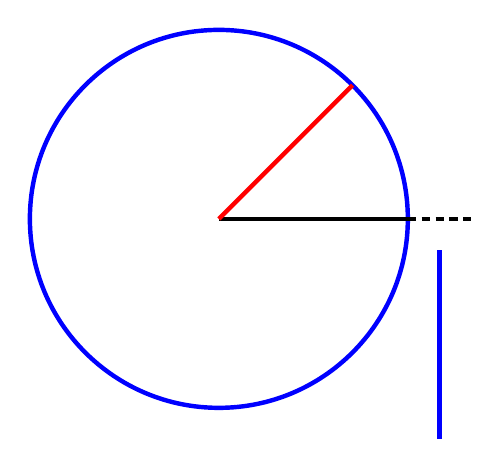
\begin{tikzpicture}[scale=0.8]
            \draw[ultra thick,blue] (0,0) circle (3cm);
            \draw[ultra thick,black] (0,0) -- (3,0);
            \draw[ultra thick,red] (0,0) -- (45:3cm);
            \draw[ultra thick,densely dashed] (3,0) -- (4,0);
            \draw[ultra thick,blue] (3.5,-0.5) -- (3.5,-3.5);
        \end{tikzpicture}
    \end{figure}

    \begin{prop}{\lettrine[lines=2]{F}rom}
		the greater (
\begin{tikzpicture} 
			\draw[ultra thick] (0,0) -- (0.9cm,0);
			\draw[densely dashed,ultra thick] (0.9cm,0) -- (1.5cm,0);
		\end{tikzpicture}
			) of two straight lines , to cut a part off equal to the less (\tikzhline[blue]{0.9cm}).\par

	\end{prop}
	\begin{proof}
		Draw $\tikzhline[red]{1cm} = \tikzhline[blue]{1cm}$ (\refprop{2}); 
        describe 
        
\begin{tikzpicture}[scale=0.5]
            \draw[ultra thick,red] (0,0) -- (45:1.15cm);
            \draw[ultra thick,blue] (0,0) circle (1cm);
        \end{tikzpicture}
        (\refpost{3}), then $\tikzhline[blue]{0.9cm} \equals \tikzhline[black]{0.9cm}.$
        \begin{align*}
            \text{For } \tikzhline[red]{0.9cm} &\equals \tikzhline[black]{0.9cm} \text{ (\refdef{15})}, \\
            \text{and } \tikzhline[blue]{0.9cm} &\equals \tikzhline[red]{0.9cm} \text{ (const.)}; \\
            \therefore\, \tikzhline[blue]{0.9cm} &\equals \tikzhline[black]{0.9cm} \text{ (\refax{1})}. 
        \end{align*}
	\end{proof}
